\documentclass[a4paper, 10pt]{article}
\usepackage[utf8]{inputenc} % Change according your file encoding
\usepackage{graphicx}
\usepackage{url}
\usepackage{amsmath}
\usepackage{mathtools}
\usepackage{mathrsfs}
\usepackage{amsfonts}
\usepackage{bbm}
\usepackage{amsthm}
\usepackage{amssymb}
\usepackage{fancyhdr}
\usepackage{setspace}
\usepackage{tabularx}
\usepackage{tikz}
\usetikzlibrary{arrows,positioning}
\usepackage[a4paper, left=2cm, right=2cm, top=2.5cm, bottom=2cm]{geometry}

\pagestyle{fancy}
\fancyhf{}
\rhead{Tuesday, December 19th}
\lhead{Víctor Mart\'in, Pablo Oviedo, and Carlos Segarra - DAG: Sheet 2}
\cfoot{\thepage}

\newtheorem{obs}{Observation}
\newtheorem{theorem}{Theorem}
\newtheorem*{theoremstar}{Theorem}

\theoremstyle{definition} % amsthm only
\newtheorem{definition}{Definition}

%\newtheorem{def}{Definition}

\newcommand{\espai}{\vspace{3mm}}
\newcommand{\cT}{\mathcal{T}}
\newcommand{\cA}{\mathcal{A}}
\newcommand{\I}{\mathscr{I}}
\newcommand{\B}{\mathscr{B}}
\newcommand{\C}{\mathscr{C}}
\newcommand{\F}{\mathscr{F}}
\newcommand{\RR}{\mathbbm{R}}
\newcommand{\aaa}{\mathbf{a}}

% Listings for Problem 5
\usepackage{listings,lstautogobble}
\definecolor{background}{rgb}{0.95,0.95,0.92}
\lstset{
    basicstyle=\footnotesize\ttfamily,
    xleftmargin=1pt,
    showstringspaces=false,
    breaklines=true,
    frame = tblr,
    autogobble = true,
    backgroundcolor=\color{background},
    commentstyle=\color{gray},
}
\lstdefinestyle{python}{
    language = Python,
    numbers = left,
    numbersep=5pt,
    keywordstyle=\color{purple},
    morekeywords={rand,timer,define},
    numberstyle=\tiny\color{gray!80},
    emphstyle=\color{red!50!blue},
    emph={addConstr, Model, addVars, GRB, gp}
}

\begin{document}
\onehalfspacing
\tikzstyle{vertice}=[circle, draw, fill=black!50, inner sep = 0pt, minimum width=4pt]

\textbf{\Large Discrete and Algorithmic Geometry: Sheet 2}

\vspace{20pt}

\textbf{\textit{(6) The permutohedron $\Pi^{n-1}$ is the convex hull of all $n!$ permutations of the vector $(1,2,\dots,n)$. For $n\ge3$, show that $\dim\Pi^{n-1}=n-1$, that $f_{n-2}(\Pi^{n-1}) = 2^n-2$, and $f_1(\Pi^{n-1}) = \tfrac12 (n-1)n!$. If you like, show that $f_k(\Pi^{n-1}) = k!\{{n\atop k}\} = \sum_{i=0}^k(-1)^i\binom{k}{i}(k-i)^n$.}}

\vspace{5pt}

WRITE HERE


\vspace{5pt}

\begin{center}
    \rule{5cm}{0.4pt}
\end{center}

\newpage

\textbf{\textit{(5) Prove (a) and (b) of the following implications for matroids, and illustrate them with a well-chosen example. Part (c) is optional and depends on your knowledge of algebra.}}

\begin{center}
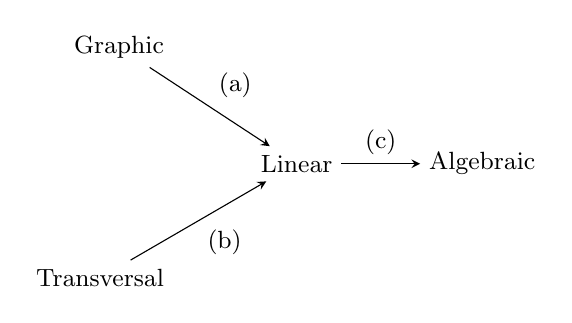
\begin{tikzpicture}\small
  \tikzset{>=stealth}
    \node (algebraic) {Algebraic};
    \node [left=of algebraic] (linear) {Linear}
    edge[->] node[above] {(c)} (algebraic) ;
    \node [above left=of linear] (graphic) {Graphic}
     edge[->] node[auto] {(a)} (linear);
     \node [below left=of linear] (transversal) {Transversal}
     edge[->] node[below right] {(b)} (linear);
  \end{tikzpicture}
\end{center}

\vspace{3pt}

We will start the proof by recalling the definitions given in class for linear, transversal, and graphical matroids.
We will define them by means of their ground set $\mathcal{E}$ and their independence sets $\mathcal{I}$.

\begin{definition}[Linear Matroid]
    Let $V$ be a vector space, then a linear matroid in $V$ is defined by
    \begin{equation*}
        \begin{split}
            \mathcal{E} & = \lbrace \text{ finite subset of } V \rbrace \\
            \mathcal{I} & = \lbrace \text{ linearly independent subsets of } \mathcal{E} \rbrace
        \end{split}
    \end{equation*}
\end{definition}

\begin{definition}[Graphical Matroid]
    Let $G = (V, E)$ be a graph,
    \begin{equation*}
        \begin{split}
            \mathcal{E} & = \lbrace \text{ edges of } G \rbrace = E \\
            \mathcal{I} & = \lbrace \text{ edges of forests of } \mathcal{G} \rbrace
        \end{split}
    \end{equation*}
\end{definition}

\begin{definition}[Transversal Matroid]
    Let $G = (U, V, E)$ be a bipartite graph,
    \begin{equation*}
        \begin{split}
            \mathcal{E} & = \lbrace \text{ bottom vertices of } G \rbrace = U \\
            \mathcal{I} & = \lbrace \text{ endpoints of maximal matchings } \mathcal{V} \rbrace
        \end{split}
    \end{equation*}
\end{definition}

To first prove (a), we want to build a linear matroid from a graphical one.
The first step is to choose our vector space, $U$.
Following the hint, let us define $U = \mathbb{R}^V$ whose standard basis is indexed by the vertices of $G = (V, E)$.
Then, if $V = \lbrace v_1, \dots, v_n \rbrace$ and $\lbrace e_{v_1}, \dots, e_{v_n}\rbrace$ is the standard basis in $U$, our ground and independence sets are defined as follows:
\begin{equation*}
    \begin{split}
        \mathcal{E} = \lbrace e_{v_i} - e_{v_j} : v_iv_j \in E \rbrace ;
        \hspace{5pt} \mathcal{I} = \bigcup_{f \text{ forest}} \lbrace e_{v_i} - e_{v_j} : v_iv_j \in E(f) \rbrace
    \end{split}
\end{equation*}
It just remains to prove that $\mathcal{I}$ as defined are indeed linearly independent subsets of $\mathcal{E}$.
Let's assume not, \textit{i.e.} one of such subset contains a linear dependence.
This is, for a forest $f$ in $G$ we have:
\begin{equation*}
    e_{v_k} - e_{v_l} = (e_{v_l} - e_{v_j}) + \dots + (e_{v_m} - e{v_n})
\end{equation*}
in this case it is clear that $k = n$ and there are two different paths to go from $v_l$ to $v_k$ what implies the existance of a cycle and hence $f$ is not a forest.
This contradicts our initial hypothesis and as a consequence $\mathcal{I}$ as defined is indeed an independence set what proves (a).

To prove (b) we will proceed in a similar manner.
In this case we have a bipartite graph $G = (E, F, H)$ where $E$ is the \textit{bottom} partition of vertices.
For our linear matroid we choose our vector space $V$ to be $\mathbbm{k}(X)^F$ with $\mathbbm{k}(X)$ defined as in the hint, and with standard basis indexed by vertices $f \in F$.
Then our ground, and independence sets are defined as follows:
\begin{equation*}
    \begin{split}
        \mathcal{E} = \left\lbrace \left\lbrace \sum_{f \in F, ef \in H} x_{e,f} u_f \right\rbrace : e \in E \right\rbrace ;
        \hspace{5pt} \mathcal{I} = \bigcup_{\text{$m$ max. matching}} \lbrace e : ef \in m, e \in E, F \in F \rbrace
    \end{split}
\end{equation*}
It just remains to prove that the sets in $\mathcal{I}$ are indeed independent.
In the same way we did for (a), we will assume some set not to be independent, hence yielding the following depndence relation:
\begin{equation*}
    \sum_{f \in F, e_1f \in H} x_{e_1,f} u_f = \sum_{f \in F, e_2f \in H} x_{e_2,f} u_f  + \dots + \sum_{f \in F, e_kf \in H} x_{e_1,f} u_f 
\end{equation*}
given that, by construction, the field extension $\mathbbm{k}(X)$ is defined by trascendentals $\lbrace x_{e,f}$, the equality can only hold iff some trascendental (\textit{e.g.} $x_{e_1,f}$ appears more than once, hence not being $m$ originally a matching in $G$.
This contradiction proves in turn (b).


\vspace{5pt}

\begin{center}
    \rule{5cm}{0.4pt}
\end{center}

\newpage

\textbf{\textit{(6) The permutohedron $\Pi^{n-1}$ is the convex hull of all $n!$ permutations of the vector $(1,2,\dots,n)$. For $n\ge3$, show that $\dim\Pi^{n-1}=n-1$, that $f_{n-2}(\Pi^{n-1}) = 2^n-2$, and $f_1(\Pi^{n-1}) = \tfrac12 (n-1)n!$. If you like, show that $f_k(\Pi^{n-1}) = k!\{{n\atop k}\} = \sum_{i=0}^k(-1)^i\binom{k}{i}(k-i)^n$.}}

\vspace{5pt}

WRITE HERE


\vspace{5pt}

\begin{center}
    \rule{5cm}{0.4pt}
\end{center}

\end{document}
